\documentclass[tikz,border=8pt]{standalone}

\usepackage[T1]{fontenc}
\usepackage[utf8]{inputenc}
\usepackage{lmodern}
\usepackage{amsmath}
\usepackage{tikz}
\usetikzlibrary{arrows.meta,positioning,fit,calc,backgrounds}

\begin{document}
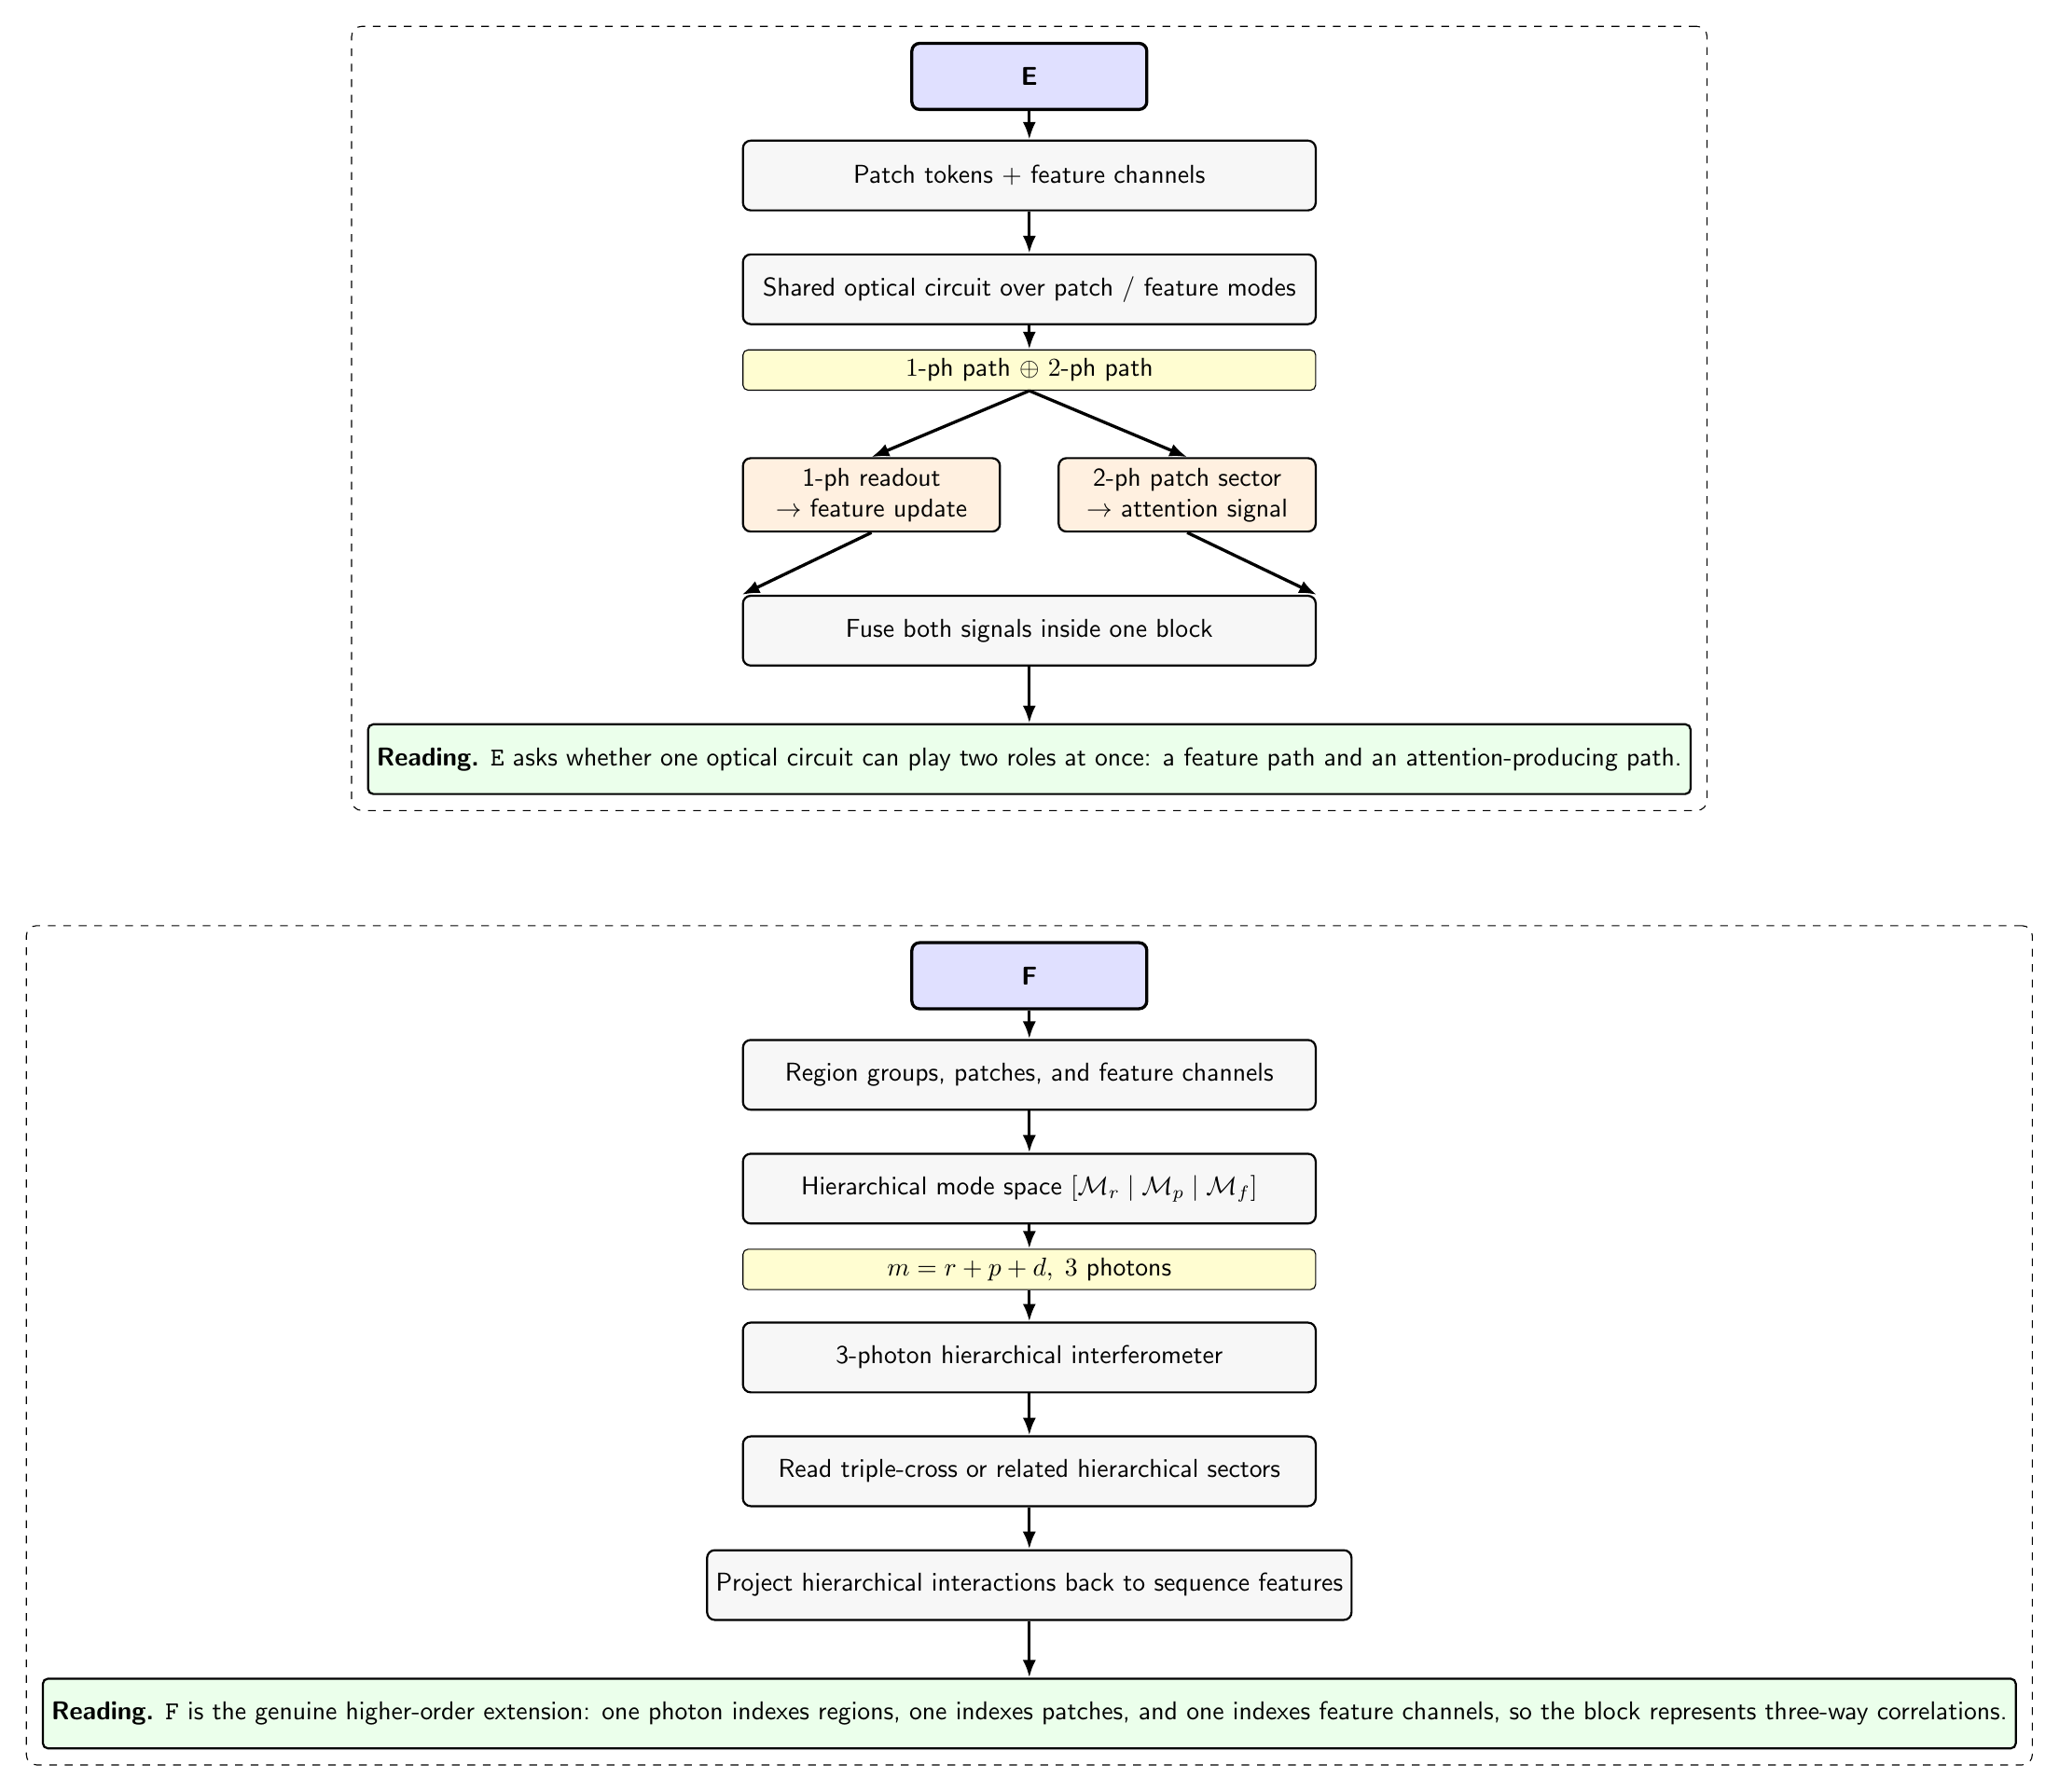
\begin{tikzpicture}[
  font=\sffamily,
  x=1cm, y=1cm,
  title/.style={draw, rounded corners=3pt, minimum width=3.2cm, minimum height=0.9cm, align=center, fill=blue!12, very thick},
  stage/.style={draw, rounded corners=3pt, minimum width=7.8cm, minimum height=0.95cm, align=center, fill=gray!6, thick},
  sector/.style={draw, rounded corners=3pt, minimum width=3.5cm, minimum height=1.0cm, align=center, fill=orange!12, thick},
  ann/.style={draw, rounded corners=2pt, minimum width=7.8cm, minimum height=0.55cm, align=center, fill=yellow!18, thin},
  note/.style={draw, rounded corners=2pt, minimum width=10.8cm, minimum height=0.95cm, align=left, fill=green!8, thick},
  arrow/.style={-{Latex[length=2.4mm]}, very thick},
  dashedbox/.style={draw, dashed, rounded corners=4pt, inner sep=6pt}
]

% E
\node[title] (etitle) at (5.5, 0.0) {\textbf{E}};
\node[stage] (e0) at (5.5, -1.35) {Patch tokens + feature channels};
\node[stage] (e1) at (5.5, -2.9) {Shared optical circuit over patch / feature modes};
\node[ann]   (ea1) at (5.5, -4.0) {$1$-ph path $\oplus$ $2$-ph path};
\node[sector] (e2) at (3.35, -5.7) {1-ph readout\\$\rightarrow$ feature update};
\node[sector] (e3) at (7.65, -5.7) {2-ph patch sector\\$\rightarrow$ attention signal};
\node[stage] (e4) at (5.5, -7.55) {Fuse both signals inside one block};
\node[note]  (en) at (5.5, -9.3) {\textbf{Reading.} \texttt{E} asks whether one optical circuit can play two roles at once: a feature path and an attention-producing path.};

% F
\node[title] (ftitle) at (5.5, -12.25) {\textbf{F}};
\node[stage] (f0) at (5.5, -13.6) {Region groups, patches, and feature channels};
\node[stage] (f1) at (5.5, -15.15) {Hierarchical mode space $[\mathcal{M}_r\mid\mathcal{M}_p\mid\mathcal{M}_f]$};
\node[ann]   (fa1) at (5.5, -16.25) {$m=r+p+d,\;3$ photons};
\node[stage] (f2) at (5.5, -17.45) {3-photon hierarchical interferometer};
\node[stage] (f3) at (5.5, -19.0) {Read triple-cross or related hierarchical sectors};
\node[stage] (f4) at (5.5, -20.55) {Project hierarchical interactions back to sequence features};
\node[note]  (fn) at (5.5, -22.3) {\textbf{Reading.} \texttt{F} is the genuine higher-order extension: one photon indexes regions, one indexes patches, and one indexes feature channels, so the block represents three-way correlations.};

\draw[arrow] (etitle.south) -- (e0.north);
\draw[arrow] (e0.south) -- (e1.north);
\draw[arrow] (e1.south) -- (ea1.north);
\draw[arrow] (ea1.south) -- (e2.north);
\draw[arrow] (ea1.south) -- (e3.north);
\draw[arrow] (e2.south) -- (e4.north west);
\draw[arrow] (e3.south) -- (e4.north east);
\draw[arrow] (e4.south) -- (en.north);

\draw[arrow] (ftitle.south) -- (f0.north);
\draw[arrow] (f0.south) -- (f1.north);
\draw[arrow] (f1.south) -- (fa1.north);
\draw[arrow] (fa1.south) -- (f2.north);
\draw[arrow] (f2.south) -- (f3.north);
\draw[arrow] (f3.south) -- (f4.north);
\draw[arrow] (f4.south) -- (fn.north);

\begin{scope}[on background layer]
  \node[dashedbox, fit=(etitle) (en)] {};
  \node[dashedbox, fit=(ftitle) (fn)] {};
\end{scope}
\end{tikzpicture}
\end{document}
